% Double-blind review copy. Shares every section file with main.tex; the only
% difference is the author block, which is anonymized here (no author names,
% no identifying artifact links), and the explicit 10pt option the IEEE
% conference template calls for. Restore paper/main.tex's real
% \author block for the camera-ready version after acceptance -- do not edit
% content sections in this file, edit the shared .tex files instead.
\documentclass[10pt,conference]{IEEEtran}
% IEEEtran sets text in Times. Under XeTeX (tectonic), Times (ptm) is not
% available, so text, bold, italics and \texttt all fell back to upright Latin
% Modern. Use the TeX Gyre clones of Times and Courier instead; pdfLaTeX builds
% are unaffected.
\usepackage{iftex}
\ifXeTeX
  \usepackage{fontspec}
  \setmainfont{texgyretermes}[Extension=.otf, UprightFont=*-regular,
    BoldFont=*-bold, ItalicFont=*-italic, BoldItalicFont=*-bolditalic]
  \setmonofont{texgyrecursor}[Extension=.otf, UprightFont=*-regular,
    BoldFont=*-bold, ItalicFont=*-italic, BoldItalicFont=*-bolditalic]
\fi
% No coloured boxes around citations and links (hyperref is loaded after this file).
\PassOptionsToPackage{hidelinks}{hyperref}


\usepackage{graphicx}
\usepackage{amsmath}
\usepackage{hyperref}
\usepackage{booktabs}
\usepackage{tabularx}
\usepackage{tikz}

% Anonymized self-citation to the companion paper (see references.bib) --
% do not cite mansy2026agentic here, it deanonymizes this submission.
\newcommand{\priorworkcite}{\cite{anon2026grammarfuzzing}}

% Anonymized artifact mirror -- do not point this at the real GitHub URL,
% it deanonymizes this submission.
\newcommand{\artifacturl}{https://anonymous.4open.science/r/agentic-fuzzing-dart-json-4656/}

\hypersetup{pdfauthor={},pdftitle={Beyond Sanitizers: LLM-Guided Refinement for Differential JSON Deserialization Testing in Dart}}

\title{Beyond Sanitizers: LLM-Guided Refinement for Differential JSON Deserialization Testing in Dart}

\author{
\IEEEauthorblockN{Anonymous Author(s)}
\IEEEauthorblockA{Submission under double-blind review}
}

% Who directed and reviewed the work (acknowledgment.tex); plural-neutral in the anonymous copy.
\newcommand{\responsibleauthor}{the author(s)}

\begin{document}

\maketitle

\begin{abstract}
A prior study of a black-box, LLM-guided grammar-fuzzing loop on native C
parsers found that the LLM writes highly valid input generators from a
grammar but that coverage-free count feedback does not improve them, and it
named a memory-safe target -- where ``crash'' has no sanitizer-based
meaning -- as future work. We take up that challenge,
retargeting the identical refinement loop at four widely-used Dart/Flutter
JSON deserialization paths (hand-written parsing, \texttt{json\_serializable},
\texttt{freezed}, and \texttt{built\_value}) and replacing the crash oracle
with two that need no crash at all: cross-implementation differential
divergence, and a ground-truth numeric round-trip check. In seeded
$n{=}5$-per-arm comparisons, the LLM's generators again raise acceptance on
a like-for-like objective (50.0\% to a 92.0\% mean, exact
$p \approx 0.0079$), and again already before any feedback arrives. On the
differential objective, however, the loop finds divergence
in only 2.9\% of generated documents against 22.2\% for a static,
schema-aware generator. Lifting the sandbox's JSON-library restriction,
richer feedback, incremental mutation, and a larger proposer model all fail
to close this gap. Giving the proposer four observations from the thirteen-case
manual characterization the static generator was designed from closes it
entirely: in a replicated comparison whose protocol was fixed in advance, refinement then reaches
a 28.8\% mean ($p \approx 0.013$ against score-only), matching the static
generator -- yet it never finds a divergence beyond what it was told. The gap
is domain knowledge, not search. The campaigns also expose two
practitioner-relevant silent failures: \texttt{json\_serializable} and
\texttt{freezed} silently saturate out-of-range integers to \texttt{int64}
bounds (649 of 11{,}449 accepted decodes each, 5.7\%), and \texttt{built\_value} silently
defaults a missing required list to empty. Maintainers confirmed both
are intended but were undocumented.

\end{abstract}

\begin{IEEEkeywords}
fuzzing, differential testing, property-based testing, large language models, JSON deserialization, Dart, Flutter, black-box testing
\end{IEEEkeywords}

\section{Introduction}

A black-box, LLM-guided grammar-fuzzing pipeline can be evaluated along two
different generalization axes. One is swapping the target implementation
while keeping everything else fixed -- a prior study did this, reusing an
identical pipeline unmodified against a second, independently implemented C
JSON parser, and found that the mechanics of the loop (harness contract,
sandbox) transferred with no redesign, and that the LLM's gain in acceptance
came from the generators it writes from the grammar, not from the count
feedback~\priorworkcite. The
other axis, which that same study named explicitly as unaddressed future
work, is swapping the \emph{oracle} itself: every component of that
pipeline's failure signal -- a sanitizer-instrumented build, a subprocess's
exit code, a fatal signal -- assumes a native process that can crash in the
memory-unsafe sense. A memory-safe language has no such crash to look for,
and ``failure'' has to be redefined around something else entirely:
uncaught exceptions, silently violated API contracts, or values that
decode incorrectly without any exception at all.

This paper takes up that second axis against a target chosen for practical
relevance: JSON deserialization in Dart, the language Flutter mobile and web
applications are written in. Porting the crash oracle onto a single,
well-audited Dart decoder would likely reproduce the uninformative negative
result the original study already reported for its second C target, so we
design two oracles that do not depend on a crash at all. The first is
\emph{differential divergence}: every generated document runs through four
widely-used Dart JSON deserialization paths --
hand-written parsing, and the \texttt{json\_serializable}, \texttt{freezed},
and \texttt{built\_value} codegen frameworks -- and disagreement between
them is the signal. The second is a \emph{ground-truth numeric round-trip
check}: JSON permits arbitrary-precision integer literals, and we check
whether a decoded value preserves the exact magnitude of the literal text
the generator wrote.

Retargeting the oracle changes what the refinement loop is asked to
optimize, and we treat that as an empirical question. \textbf{RQ1}: reusing
the original acceptance-rate proxy and loop essentially unmodified, does
LLM-guided refinement still raise a Dart JSON generator's rate of producing
syntactically valid documents? \textbf{RQ2}: does malformed or
boundary-case input surface divergence across the four paths, and does
refinement -- with its prompt corrected to make divergence the explicit
objective -- find more of it than a static, schema-aware generator?
\textbf{RQ3}: does numeric decoding preserve exact integer values at
magnitudes JSON permits but native integer types do not, measured at scale?

We answer RQ1 affirmatively and RQ2 negatively. The same loop, proposer
model, and iteration budget succeed on one objective and not on the other,
and the difference is what the model already knows: it writes valid JSON
generators without any feedback, but it does not know where four Dart
deserializers disagree. We then trace the RQ2 gap to exactly that: not the
loop's ability to search, but the domain knowledge the static generator's
designer had and the loop did not. This paper contributes:

\begin{itemize}
  \item Two coverage-free, crash-free oracles for a memory-safe target --
    cross-implementation differential divergence and ground-truth numeric
    round-tripping -- and a two-stage harness (a shared JSON-syntax gate,
    then four independent schema-level decodes) that computes them
    automatically.
  \item A seeded $n{=}5$-per-arm replication (RQ1) showing the LLM's
    generators reproduce the acceptance gain on a new runtime and language
    (50.0\% to a 92.0\% mean, exact two-sided $p \approx 0.0079$), with
    the generators written before any feedback already the most valid.
  \item A comparison (RQ2) showing the same mechanism \emph{underperforms} a
    static generator by an order of magnitude on the divergence objective
    (2.9\% vs.\ 22.2\% mean, $p \approx 0.0079$), and three follow-ups that
    test rather than assume the reason: removing generation overhead
    (\texttt{import json} allowed) leaves the rate unchanged, richer
    category feedback makes it worse ($p \approx 0.032$ uncorrected), and
    mutate-not-rewrite refinement does not replicate a promising held-out
    seed -- localizing the gap to targeting.
  \item A replicated knowledge-parity experiment, with its protocol fixed in advance, showing the
    gap is domain knowledge: given four observations from a thirteen-case
    manual characterization, refinement matches the static generator
    (28.8\% mean, $p \approx 0.013$ against score-only), while a larger
    proposer without them does not improve (\texttt{gpt-4.1}, 1.91\%,
    $p \approx 0.31$) -- and the loop never finds divergence beyond what it
    was told.
  \item A methodological note: an initial prompt found \emph{zero}
    divergence across three full seeded runs while driving up unrelated
    rejection counts; a principled revision, first tried on one fresh seed
    before further spend, recovered a consistent effect. We report the
    failed design alongside the fix.
  \item Two practitioner-relevant silent failures found with no LLM involved and
    confirmed at scale (RQ3): \texttt{json\_serializable}/\texttt{freezed}
    silently saturate out-of-range integers to \texttt{int64} bounds (649 of
    11{,}449 accepted decodes each, 5.7\%), and \texttt{built\_value} silently
    defaults a missing required list to empty -- plus a released pipeline,
    harness, and full campaign artifact set.
\end{itemize}

\section{Related Work}
\label{sec:related-work}

\paragraph{Coverage-guided fuzzing}
American Fuzzy Lop~\cite{zalewski2014afl} and its successor AFL++~\cite{fioraldi2020aflplusplus}
popularized mutation-based, coverage-guided fuzzing: a target is
instrumented to report which code ran, and the fuzzer retains and mutates
inputs that reach new coverage. Man\`es et al.'s survey~\cite{manes2021fuzzing}
gives a taxonomy of this and related approaches. Coverage-guided fuzzers are
highly effective when instrumentation is available, but instrumentation
itself is exactly what a memory-safe, JIT/AOT-compiled runtime such as
Dart's makes both less necessary (there is no memory-safety class of bug for
a sanitizer to catch) and less available in the form these tools assume;
none of this family targets the failure modes this paper is concerned with.

\paragraph{Grammar-based and generation-based fuzzing}
Generating inputs directly from a grammar, rather than mutating bytes, is a
much older idea: Purdom's sentence generator~\cite{purdom1972sentence}
produces short strings that exercise every grammar production, originally
for testing and debugging parsers themselves. More recent tools combine a
grammar with coverage feedback: Superion~\cite{wang2019superion} extends a
greybox fuzzer with grammar-aware mutation operators so mutated inputs
remain syntactically valid, and Nautilus~\cite{aschermann2019nautilus}
similarly pairs a grammar-based generator with coverage-guided mutation to
reach deeper parser states. Both still assume coverage instrumentation is
available; the pipeline this paper extends removes that assumption
entirely.

\paragraph{Property-based testing}
QuickCheck~\cite{claessen2000quickcheck} introduced property-based testing:
a developer writes generators for values of a given shape and a property
that should hold for all of them, and the tool searches for a
counterexample. Hypothesis~\cite{maciver2019hypothesis}, which the pipeline
this paper reuses builds directly on, is a Python implementation of the
same idea, with composable strategies expressive enough to encode both a
formal grammar (our RQ1 generator) and an adversarial perturbation catalog
over a target-specific schema (our RQ2 generator, Section~\ref{sec:methodology}).

\paragraph{LLMs for fuzzing and test generation}
LLMs have recently been used to generate or mutate fuzzing inputs directly.
TitanFuzz~\cite{deng2023titanfuzz} uses an LLM to generate and mutate
programs for fuzzing deep-learning library APIs, relying on the LLM's prior
exposure to real usage examples of those APIs rather than a formal grammar.
Fuzz4All~\cite{xia2024fuzz4all} generalizes this to arbitrary
languages/systems by using an LLM both to synthesize a distilled input
prompt from documentation and examples and to generate and mutate inputs
from it. CodaMOSA~\cite{lemieux2023codamosa} invokes an LLM only after
search-based test generation's coverage plateaus, asking it for example
test cases to escape the plateau -- i.e., the LLM is invoked \emph{because}
coverage feedback is available and has stalled. G2Fuzz~\cite{zhang2025g2fuzz}
and ELFuzz~\cite{chen2025elfuzz} have an LLM synthesize and evolve input
generators, but select them by coverage. This paper's setting differs
along the same axis as its predecessor~\priorworkcite: no coverage
signal is available at any point, and the LLM's job is to revise a reusable,
executable \emph{generator} against feedback a black-box harness can
actually produce, not to emit one-off inputs.

\paragraph{Differential testing}
Running multiple independent implementations of the same specification
against identical inputs and comparing their outputs, rather than checking
each against a hand-written oracle, dates to McKeeman's differential
testing~\cite{mckeeman1998differential}. This idea is what makes RQ2's
oracle possible at all in a setting with no crash to detect: four
Dart JSON deserialization paths (three of them independently implemented) sharing one
formal schema give a comparison target for free, the same way McKeeman
compared independent compiler implementations against each other rather
than against a formal semantics. Where classic differential testing
compares whole programs given the same input, our four paths share almost
their entire input pipeline (Section~\ref{sec:methodology}'s shared
JSON-syntax gate) and differ only in schema-level decoding, which is a
narrower and, we find, more failure-prone surface than differential testing
is usually applied to. For JSON specifically, cross-language differential
testing of parsers has found many semantic discrepancies at the text-to-tree
level~\cite{moller2024crosslanguage}, and JsonATG~\cite{wang2025jsonatg} uses
a multi-agent LLM pipeline to generate bug-triggering tests for Java JSON
libraries; we instead target typed binding, from tree to class, where all four
paths share the parsing step. With an LLM in the loop,
Mokav~\cite{etemadi2025mokav} feeds the outputs of two program versions back
to the model until it finds a difference-exposing input; our loop receives
only a divergence score, which RQ2's follow-ups vary.

\paragraph{Positioning} This paper is a direct empirical follow-up to
\priorworkcite, which evaluated the identical refinement-loop
mechanism on two independently implemented C JSON parsers under a
sanitizer-based crash oracle and named a memory-safe target as future work
along a materially different generalization axis. We take up exactly that
axis: same loop, same sandboxing discipline, same reproducibility tooling
where none of it is C- or format-specific, retargeted at a language where
the entire premise of a crash oracle does not hold, using differential
divergence~\cite{mckeeman1998differential} and ground-truth numeric
round-tripping as replacements. Unlike TitanFuzz, Fuzz4All, and CodaMOSA,
the LLM here never sees coverage data, execution traces, or usage examples --
only a schema description and the same three-signal proxy discipline (here,
a divergence score in place of acceptance rate) a human maintaining a
Hypothesis strategy by hand would have to reason about manually.

\section{Methodology}
\label{sec:methodology}

\subsection{Research questions}
RQ1: reusing the original acceptance-rate proxy and refinement loop
unmodified in mechanism, does LLM-guided refinement raise the fraction of
generated documents a Dart JSON decoder accepts as syntactically valid,
relative to the static baseline, as it did for a native C
target? RQ2: across four widely-used Dart JSON deserialization
paths, does malformed or boundary-case input surface behavioral divergence,
and does refinement -- once its prompt is corrected to make divergence the
explicit objective -- find more of it than a static, schema-aware generator?
RQ3: does numeric decoding across these paths preserve exact integer values
at magnitudes JSON permits syntactically but a 64-bit integer type does not,
and how does this generalize once measured at scale?

\subsection{Target set}
\label{sec:target-set}
Four Dart~\cite{dart2026lang} JSON deserialization paths over one shared
schema (Section~\ref{sec:schema}), chosen for being how a real Flutter
codebase actually deserializes JSON today, not for novelty: (A)
hand-written parsing via \texttt{dart:convert}'s \texttt{jsonDecode} plus
explicit \texttt{as} casts, representing code with no generated safety net;
(B) \texttt{json\_serializable}~6.14.1~\cite{jsonserializable2026}, the most
widely used Dart codegen serialization package; (C)
\texttt{freezed}~4.0.1~\cite{freezed2026}, configured to delegate JSON
leaf-decoding to \texttt{json\_serializable} so that any B-vs-C divergence
is attributable to freezed's own contribution (immutability, union
discrimination) rather than a second independent JSON decoder; (D)
\texttt{built\_value}~8.13.0~\cite{builtvalue2026}, an
independently-designed, typed-serializer-based model rather than an
annotation-and-\texttt{Map}-based one like B/C, and consequently the path
most likely to diverge for genuinely independent-implementation reasons.
All four resolve together under one Dart~3.13.2 toolchain with no
dependency conflicts; exact versions are pinned in a committed lockfile.

\subsection{Shared schema}
\label{sec:schema}
One logical record, hand-implemented once per path: \texttt{id} (a bare JSON
integer, RQ3's target field), \texttt{amount} (a JSON string, carrying text
byte-for-byte with no numeric coercion by any path, so it cannot exhibit
RQ3's failure mode -- it exists purely to widen RQ2's perturbation surface),
\texttt{name} (nullable string), \texttt{status} (one of three enumerated
string values, chosen to probe unrecognized-enum-value handling), \texttt{tags}
(a list of strings), and \texttt{child} (one bounded level of recursive
nesting of the same record).

\subsection{Two coverage-free, crash-free oracles}
\label{sec:oracles}
Every generated document passes through a two-stage harness. \textbf{Stage
one, a shared structural gate}: base64-decode the candidate bytes, decode as
UTF-8, then attempt \texttt{jsonDecode}. Any failure here -- invalid UTF-8,
invalid JSON syntax, or a syntactically valid but non-object top-level value
(a bare array, number, or \texttt{null}, which JSON's grammar permits but no
path can schema-decode) -- is recorded once, uniformly, since all four paths
share this exact entry point and would fail identically before ever
diverging. This has a direct consequence for generator design
(Section~\ref{sec:generators}): a byte-level, grammar-only mutator can vary
only what this shared gate tests, so it cannot find divergence by
construction -- divergence can only exist at the schema stage. \textbf{Stage
two, four independent schema attempts}, reached only if stage one succeeds:
each of the four paths attempts to decode the same parsed object,
independently caught so that one path's exception can never prevent the
other three from running on the same input. Each result is either
\emph{accepted}, with a canonical value (Section~\ref{sec:canonical}), or
\emph{rejected}, with the concrete runtime type of the exception and whether
that type is \emph{private} -- Dart's leading-underscore naming convention
marking a class as internal to its defining library, meaning calling code
cannot name it in a \texttt{catch} clause and must catch a generic
supertype instead. This operationalizes ``undocumented failure surface''
mechanically rather than via a hand-maintained list of each package's
documented exceptions.

From these four records, two divergence-based oracles are computed
automatically, with no crash required: \textbf{cross-path divergence}
(RQ2) is \emph{accept/reject} when acceptance status differs across paths,
or \emph{value} when two or more accepting paths decode to different
canonical values. \textbf{Numeric round-trip divergence} (RQ3) compares each
accepting path's canonical \texttt{id} against the exact ground-truth
integer parsed from the candidate's own source text -- Python's arbitrary-precision
\texttt{int} serializes exactly via \texttt{json.dumps} with no
\texttt{float} detour, so ground truth requires no special-cased generation,
only ordinary integer drawing at a biased range. A genuine process-level
fault (the harness killed by a signal, or a batch timeout) is this
pipeline's closest analogue to the original's sanitizer-based crash tier,
checked around a whole campaign rather than around one input
(Section~\ref{sec:harness-arch}).

\subsection{Canonical value comparison}
\label{sec:canonical}
Comparing decoded values safely requires that comparison itself not
reintroduce the exact class of error the oracle exists to detect. Each
path's typed result is converted, once, to a shared representation using
only Dart primitives -- strings, exact-precision integers, booleans,
\texttt{null}, and nested maps/lists -- and compared structurally, never as
a floating-point value. Any reported divergence is therefore real by
construction, not an artifact of the comparison logic.

\subsection{Harness architecture}
\label{sec:harness-arch}
The original pipeline spawns one process per input, which is cheap for a
single native binary but would be four times as expensive here and
provides no fault-isolation benefit a memory-safe language cannot already
give in-process (an exception is caught, not a process-ending fault, unless
truly fatal). The harness is instead one AOT-compiled, long-lived process
per campaign, reading newline-delimited JSON requests from stdin -- one
line per candidate, base64-encoded since a candidate may be invalid UTF-8 by
design -- and writing one newline-delimited JSON result per line, flushed
immediately so a driver can still attribute a later process-level fault to
the correct input despite one process now serving an entire campaign rather
than one input.

\subsection{Generators}
\label{sec:generators}
\textbf{RQ1} reuses the original pipeline's static baseline completely
unmodified: it alternates a bounded JSON value serialized with Python's
\texttt{json.dumps} with the same document plus one malformed suffix, so
exactly half its inputs are invalid by design. The proposer is given the
ANTLR grammars-v4 JSON grammar~\cite{antlr2024grammarsv4,parr2013antlr}.
RQ1 targets the shared structural gate directly:
``accepted'' is defined exactly as the original grammar defines it -- any
value type at the top level, not only objects -- specifically so this
research question tests portability of the loop on a
like-for-like criterion, not a criterion this paper's own schema happens to
impose. \textbf{RQ2/RQ3} require a schema-aware generator instead, since
Section~\ref{sec:oracles}'s shared gate makes a grammar-only mutator
structurally incapable of finding schema-level divergence: a base
valid-record generator draws each field at its correct type, with
\texttt{id} biased toward magnitudes near \texttt{double}'s exact-integer
boundary and 64-bit integer boundaries; an independently-probable
perturbation layer then drops a field, substitutes a wrong-but-JSON-valid
type, nulls a field regardless of nullability, substitutes an out-of-enum
string, injects an unknown key, or forces deeper recursion than the base
generator's normal cap. For the LLM-refined arm, the identical
\texttt{@st.composite def generated\_json(draw) -> bytes} contract is used,
with a schema description substituted for the grammar text in the prompt
and, for RQ2, a divergence score (Section~\ref{sec:rq2-prompt}) in place of
acceptance rate as the quantity the prompt asks the model to maximize.

\subsection{What transfers unmodified from the original pipeline}
The original project's AST-based sandbox over LLM-authored proposals
(import restricted to \texttt{hypothesis.strategies}, a blocklist over
named code-execution/I-O entry points, and a behavioral sanity check that
the proposal actually produces \texttt{bytes}); its bounded iteration
budget and error-recovery discipline (a failing proposal consumes an
iteration slot and its exact error text is fed into the next prompt, rather
than aborting the run); its Hypothesis reproducibility shim (pinned to the exact
Hypothesis version whose private internal it patches); and its per-iteration
artifact discipline (every prompt, proposal, and result persisted, nothing
discarded) are all reused with no logic changes, only the target-specific
campaign runner beneath them replaced. The structural-fingerprint
diversity proxy is likewise reused verbatim: it is JSON-specific, not
C-specific, and the format has not changed.

\subsection{RQ2's refinement prompt: a confirmed fix, not a guess}
\label{sec:rq2-prompt}
An initial prompt presented the divergence count alongside per-path
rejection counts in one undifferentiated metrics object, with no relative
weighting. Across three full seeded runs this produced zero divergence
despite driving rejection counts up sharply -- confirmed as systematic,
not run-to-run noise, before any prompt change was made
(Section~\ref{sec:evaluation-rq2}). The prompt was revised to state an
explicit numeric score (divergence count over total), to say plainly that a
high rejection count alone is not the goal, and to add a methodological
hint -- vary one or two things about an otherwise-valid document rather
than maximizing how broadly malformed a document looks -- deliberately
worded to avoid naming the specific fields or outcomes already known by
hand, so that any resulting discovery would be the loop's own. The fix was
first run on one fresh seed (seed 3) before being adopted; that run is one
of the five reported score-only runs (Section~\ref{sec:evaluation-rq2}).

\subsection{Follow-up arms on the RQ2 gap}
\label{sec:ablation-json}\label{sec:category-feedback}\label{sec:mutate-source}
Five further refined arms, each on fresh seeds disjoint from every other
run and otherwise identical to the main refined arm, test why refinement
underperforms on RQ2. \textbf{JSON allowed} (seeds 100--104): the sandbox
forbids importing \texttt{json}, forcing the LLM to hand-build JSON text; this
arm permits \texttt{import json} (via a separate sandbox module, so the
original validator is never modified), isolating generation overhead from
targeting. \textbf{Category feedback} (seeds 200--204): in addition to the
score, the prompt reports how many divergence-causing documents exhibited
each perturbation category -- missing field, null override, wrong type,
unrecognized enum, boundary-magnitude \texttt{id}, extra key, deep nesting --
classified automatically from each document's shape and never naming
specific fields, preserving Section~\ref{sec:rq2-prompt}'s discipline
against planting the answer. \textbf{Mutate source} (seeds 400--404): every
other arm discards the previous iteration's generator; this one shows the
proposer its own previous source and asks it to revise it incrementally.
Because a held-out seed showed a buggy revision persisting for the rest of
a run, it carries a revert-on-regression guard: if the syntactically valid
fraction drops more than 10 percentage points below the run's best so far,
the next iteration mutates from the best-known source instead, with a note
telling the proposer what regressed.

\textbf{Knowledge parity} (seeds 500--509)\label{sec:knowledge-parity}: the
static generator's perturbation catalog was designed after the thirteen-case
characterization of the four paths (documents chosen by the researchers and
run through the harness outside the loop), while every refined arm above sees only
the schema and its score. This arm adds to the score-only prompt exactly what
that designer knew beforehand, as four plain observations with no generator
code: invalid JSON is rejected identically by all four paths;
\texttt{built\_value} accepts a missing \texttt{tags} while the others
reject it; wrong types, nulls, and unknown enum values are rejected by all
four, while extra keys and missing nullable fields are accepted by all four;
and \texttt{json\_serializable}/\texttt{freezed} decode \texttt{id} via
\texttt{(json['id'] as num).toInt()}, which saturates out-of-range values.
\textbf{Stronger proposer} (seeds 605--609): the score-only arm with
\texttt{gpt-4.1} in place of \texttt{gpt-4.1-mini} -- same family, same API
parameters, not a reasoning model -- testing whether a more capable model
discovers that knowledge from the score alone. Because \texttt{gpt-4.1}
routinely appends prose after its fenced code block, which the original
response parser does not strip (a first run on seeds 600--604 lost 11 of 25
iterations to this), this arm extracts the first fenced block; the fix is
opt-in, affected at most 2 iterations of any \texttt{gpt-4.1-mini} arm, and
favors \texttt{gpt-4.1}. For both arms, seeds, tests, and decision rules were
written into the released design document before any run.

\subsection{Experimental design}
All three research questions use seeded, independent runs (Hypothesis's
draw stream reseeded once per run via the reproducibility shim above), with
$n{=}5$ per arm under a fixed API budget, reported as such throughout --
the same discipline the original project applied to its own smaller-sample
ablation. RQ1 compares the static baseline (one campaign of 500
examples per run) against five refined runs (five iterations of up
to 500 examples each, \texttt{gpt-4.1-mini}, temperature 0.2). RQ2 compares
a static baseline (the schema-aware generator, one campaign of 500
examples per run) against five refined runs under the corrected prompt.
RQ3 requires no separate campaign: every schema-evaluated record collected
for RQ2 already carries each path's canonical \texttt{id} and the
document's own source text, so RQ3's ground-truth comparison is computed as
an analysis pass over RQ2's existing campaign data rather than a third parallel
generator/harness/campaign pipeline.

\section{Evaluation}
\label{sec:evaluation}

All reported $p$-values are exact, two-sided Mann-Whitney U tests
(\texttt{scipy.stats.mannwhitneyu}, \texttt{method="exact"}). At $n{=}5$ per
arm, $C(10,5) = 252$ and exactly two partitions produce complete rank
separation, so $p = 2/252 \approx 0.00794$ in every complete-separation case
below -- the smallest $p$ this design can produce, not a coincidence between
unrelated effects.

\subsection{RQ1: does the acceptance gain transfer?}
\label{sec:evaluation-rq1}
Table~\ref{tab:rq1} reports acceptance rate -- the fraction of generated
documents that are syntactically valid JSON by the same criterion the
original grammar uses, any value type at the top level -- for five seeded
baseline runs and five seeded refined runs. The baseline is exactly 50.0\%
on every run by construction (its input stream deterministically alternates
a grammar-valid generator with a deliberately corrupted variant of it).
Every refined run exceeds every baseline run: complete rank separation,
exact $p \approx 0.00794$. One refined run's lower rate (68.6\%, seed 0)
traces to its fourth-iteration generator, which deliberately emitted
malformed \texttt{\textbackslash u} escapes to keep near-valid cases, as the
prompt asks; 300 of its 500 documents were rejected. Across the five runs, 14
of 25 proposals failed validation, through ordinary LLM code-generation errors
(e.g.\ one built an unbounded-depth strategy that hit Python's recursion
limit), and were logged and handled as the original pipeline's
error-recovery design specifies.

\begin{table}[t]
\centering
\footnotesize
\caption{RQ1: acceptance rate, $n{=}5$ seeded runs per arm.}
\label{tab:rq1}
\begin{tabularx}{\columnwidth}{@{}lX@{}}
\toprule
Metric & Value \\
\midrule
Baseline, per-run (\%) & 50.0, 50.0, 50.0, 50.0, 50.0 \\
Refined, per-run (\%) & 68.6, 97.3, 98.0, 98.1, 98.2 \\
Baseline mean (stdev) & 50.0 (0.0) \\
Refined mean (stdev) & 92.0 (13.1) \\
\bottomrule
\end{tabularx}
\end{table}

This reproduces the original study's cJSON result in shape -- 58.2\% to
97.1\% there, 50.0\% to a 92.0\% mean here -- on a different runtime and
language, and it shares that result's explanation. Of the iterations that
produced data, the five whose prompt had not yet carried any campaign result
(they came first, or followed only failed proposals) accepted 98.3\% of
their documents, and the six written after feedback accepted 87.8\%,
including seed 0's deliberately near-valid generator. In the prior study, a
pre-registered arm that never saw feedback matched the refined
arm~\priorworkcite; here too, the gain is the model's own: given the
grammar, it writes a generator of valid JSON. The baseline's 50.0\% is a
design choice, since half its inputs are malformed on purpose. RQ1 thus
establishes that the loop works end to end on the new harness, and that
producing valid JSON is not where its difficulty lies.

\subsection{RQ2: does refinement find more divergence than a static generator?}
\label{sec:evaluation-rq2}
The first refinement prompt (Section~\ref{sec:rq2-prompt}) was run across
three full seeded runs (seeds 0--2) before any revision: zero cross-path
divergence in every resulting iteration-campaign, despite per-path rejection
counts climbing sharply (up to 208 of 264 schema-evaluated documents on one
run). The revised prompt was first run on one fresh seed, seed 3 (11.8\%
divergence in its best iteration), before being adopted; seed 3 is one of
the five score-only runs in Table~\ref{tab:rq2}, and its best one (5.53\%).
Excluding it lowers the score-only mean to 2.28\% and changes no
conclusion below: the static baseline still separates completely
($p \approx 0.016$, the minimum for five against four runs), and knowledge
parity stays significant ($p \approx 0.024$).

\begin{table}[t]
\centering
\footnotesize
\caption{RQ2: cross-path divergence rate (\% of all generated documents), seeded runs per arm ($n{=}5$ unless noted). $p$: exact two-sided Mann-Whitney U against the score-only refined arm. Every arm except parity is in complete separation below the static baseline ($p \approx 0.0079$). $^{*}$Knowledge parity, $n{=}10$.}
\label{tab:rq2}
\setlength{\tabcolsep}{3pt}
\begin{tabularx}{\columnwidth}{@{}lXrr@{}}
\toprule
Arm & Per-run (\%) & Mean (sd) & $p$ \\
\midrule
Static baseline & 19.8, 21.8, 22.2, 23.4, 23.8 & 22.2 (1.57) & 0.0079 \\
Score-only & 1.3, 1.45, 2.75, 3.6, 5.53 & 2.93 (1.74) & -- \\
\quad JSON allowed & 0.05, 2.2, 2.36, 2.36, 4.05 & 2.20 (1.42) & 0.69 \\
\quad Categories & 0.0, 0.0, 1.0, 1.2, 2.55 & 0.95 (1.05) & 0.032 \\
\quad Mutate source & 0.0, 0.30, 0.65, 2.93, 4.75 & 1.73 (2.05) & 0.31 \\
\quad \texttt{gpt-4.1} & 0.0, 0.36, 0.60, 2.52, 6.05 & 1.91 (2.51) & 0.31 \\
\quad Parity$^{*}$ & 0.0, 17.6, 22.1, 26.4, 27.7, 31.0, 36.6, 38.7, 41.6, 45.9 & 28.8 (13.45) & 0.013 \\
\bottomrule
\end{tabularx}
\end{table}

\begin{figure}[t]
\centering
% Generated by scripts/make_strip_figure.py from artifacts/repeated; do not edit.
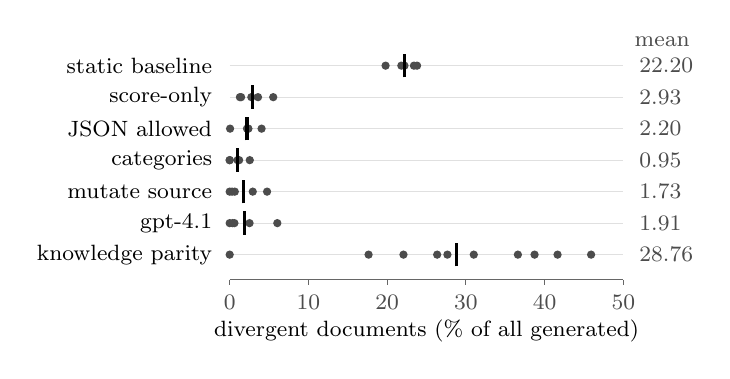
\begin{tikzpicture}[font=\footnotesize]
\node[anchor=east] at (-0.1,0.00) {static baseline};
\draw[black!12] (0,0.00) -- (5.0,0.00);
\fill[black!70] (1.980,0.00) circle (1.5pt);
\fill[black!70] (2.180,0.00) circle (1.5pt);
\fill[black!70] (2.220,0.00) circle (1.5pt);
\fill[black!70] (2.340,0.00) circle (1.5pt);
\fill[black!70] (2.380,0.00) circle (1.5pt);
\draw[black, line width=1.1pt] (2.220,-0.15) -- (2.220,0.15);
\node[anchor=west, black!70] at (5.08,0.00) {22.20};
\node[anchor=east] at (-0.1,-0.40) {score-only};
\draw[black!12] (0,-0.40) -- (5.0,-0.40);
\fill[black!70] (0.553,-0.40) circle (1.5pt);
\fill[black!70] (0.130,-0.40) circle (1.5pt);
\fill[black!70] (0.145,-0.40) circle (1.5pt);
\fill[black!70] (0.275,-0.40) circle (1.5pt);
\fill[black!70] (0.360,-0.40) circle (1.5pt);
\draw[black, line width=1.1pt] (0.293,-0.55) -- (0.293,-0.25);
\node[anchor=west, black!70] at (5.08,-0.40) {2.93};
\node[anchor=east] at (-0.1,-0.80) {JSON allowed};
\draw[black!12] (0,-0.80) -- (5.0,-0.80);
\fill[black!70] (0.236,-0.80) circle (1.5pt);
\fill[black!70] (0.005,-0.80) circle (1.5pt);
\fill[black!70] (0.405,-0.80) circle (1.5pt);
\fill[black!70] (0.236,-0.80) circle (1.5pt);
\fill[black!70] (0.220,-0.80) circle (1.5pt);
\draw[black, line width=1.1pt] (0.220,-0.95) -- (0.220,-0.65);
\node[anchor=west, black!70] at (5.08,-0.80) {2.20};
\node[anchor=east] at (-0.1,-1.20) {categories};
\draw[black!12] (0,-1.20) -- (5.0,-1.20);
\fill[black!70] (0.000,-1.20) circle (1.5pt);
\fill[black!70] (0.100,-1.20) circle (1.5pt);
\fill[black!70] (0.255,-1.20) circle (1.5pt);
\fill[black!70] (0.000,-1.20) circle (1.5pt);
\fill[black!70] (0.120,-1.20) circle (1.5pt);
\draw[black, line width=1.1pt] (0.095,-1.35) -- (0.095,-1.05);
\node[anchor=west, black!70] at (5.08,-1.20) {0.95};
\node[anchor=east] at (-0.1,-1.60) {mutate source};
\draw[black!12] (0,-1.60) -- (5.0,-1.60);
\fill[black!70] (0.000,-1.60) circle (1.5pt);
\fill[black!70] (0.293,-1.60) circle (1.5pt);
\fill[black!70] (0.475,-1.60) circle (1.5pt);
\fill[black!70] (0.065,-1.60) circle (1.5pt);
\fill[black!70] (0.030,-1.60) circle (1.5pt);
\draw[black, line width=1.1pt] (0.173,-1.75) -- (0.173,-1.45);
\node[anchor=west, black!70] at (5.08,-1.60) {1.73};
\node[anchor=east] at (-0.1,-2.00) {gpt-4.1};
\draw[black!12] (0,-2.00) -- (5.0,-2.00);
\fill[black!70] (0.060,-2.00) circle (1.5pt);
\fill[black!70] (0.252,-2.00) circle (1.5pt);
\fill[black!70] (0.605,-2.00) circle (1.5pt);
\fill[black!70] (0.000,-2.00) circle (1.5pt);
\fill[black!70] (0.036,-2.00) circle (1.5pt);
\draw[black, line width=1.1pt] (0.191,-2.15) -- (0.191,-1.85);
\node[anchor=west, black!70] at (5.08,-2.00) {1.91};
\node[anchor=east] at (-0.1,-2.40) {knowledge parity};
\draw[black!12] (0,-2.40) -- (5.0,-2.40);
\fill[black!70] (4.590,-2.40) circle (1.5pt);
\fill[black!70] (2.207,-2.40) circle (1.5pt);
\fill[black!70] (0.000,-2.40) circle (1.5pt);
\fill[black!70] (3.660,-2.40) circle (1.5pt);
\fill[black!70] (1.764,-2.40) circle (1.5pt);
\fill[black!70] (4.164,-2.40) circle (1.5pt);
\fill[black!70] (2.635,-2.40) circle (1.5pt);
\fill[black!70] (3.872,-2.40) circle (1.5pt);
\fill[black!70] (3.100,-2.40) circle (1.5pt);
\fill[black!70] (2.765,-2.40) circle (1.5pt);
\draw[black, line width=1.1pt] (2.876,-2.55) -- (2.876,-2.25);
\node[anchor=west, black!70] at (5.08,-2.40) {28.76};
\draw[black!60] (0,-2.72) -- (5.0,-2.72);
\draw[black!60] (0.000,-2.72) -- (0.000,-2.79);
\node[anchor=north, black!70] at (0.000,-2.79) {0};
\draw[black!60] (1.000,-2.72) -- (1.000,-2.79);
\node[anchor=north, black!70] at (1.000,-2.79) {10};
\draw[black!60] (2.000,-2.72) -- (2.000,-2.79);
\node[anchor=north, black!70] at (2.000,-2.79) {20};
\draw[black!60] (3.000,-2.72) -- (3.000,-2.79);
\node[anchor=north, black!70] at (3.000,-2.79) {30};
\draw[black!60] (4.000,-2.72) -- (4.000,-2.79);
\node[anchor=north, black!70] at (4.000,-2.79) {40};
\draw[black!60] (5.000,-2.72) -- (5.000,-2.79);
\node[anchor=north, black!70] at (5.000,-2.79) {50};
\node[anchor=north] at (2.50,-3.10) {divergent documents (\% of all generated)};
\node[anchor=south west, black!70] at (5.02,0.12) {mean};
\end{tikzpicture}

\caption{RQ2 divergence rate of every run (dots: seeds; bar and number:
mean). Every intervention without domain knowledge stays near the
score-only arm; four observations from the manual characterization lift
the loop to the static baseline's level.}
\label{fig:rq2-strip}
\end{figure}

Every baseline run exceeds every refined run (Fig.~\ref{fig:rq2-strip}): complete rank separation,
exact $p \approx 0.00794$, in the opposite direction from RQ1. Part of the
gap is generation overhead -- the sandbox forbids importing a JSON library,
so the LLM hand-builds JSON text, and the refined arm's schema-evaluated
fraction ranged 41.9\%--83.7\% across runs versus the baseline's fixed
100\% -- but restricting to schema-evaluated documents still leaves 4.10\%
against 22.2\%. Pooling every schema-evaluated record across the five
refined seeds, the loop found exactly the same two divergence patterns the
static generator found -- the two silent failures in
Section~\ref{sec:evaluation-defects} -- never a qualitatively new one, at a
lower rate throughout.

\subsection{Why does refinement underperform? Three follow-ups}
\label{sec:evaluation-ablation}\label{sec:evaluation-category-feedback}\label{sec:evaluation-mutate-source}
The lower rows of Table~\ref{tab:rq2} report the three follow-up arms of
Section~\ref{sec:ablation-json}.

\textbf{Generation overhead or targeting?} With \texttt{import json}
permitted, every one of the 24 iterations that produced data reached 100\%
(in one case, affected by an unrelated encoding issue, 82.5\%)
schema-evaluated output -- the overhead is essentially eliminated -- yet
the divergence rate did not improve: 2.20\% mean, statistically
indistinguishable from the constrained sandbox ($p \approx 0.69$). Removing
the overhead entirely closes no measurable part of the gap; the shortfall
is a targeting problem.

\textbf{Does richer feedback help?} Category feedback did measurably
\emph{worse}: 0.95\% mean against the score-only prompt's 2.93\%, both over
all documents and restricted to schema-evaluated ones ($p \approx 0.032$ in
each case, ruling out proposal-failure noise; 0.13 after a Holm correction
across the four exploratory follow-ups). Two of the five seeds found
zero divergence in their only successfully validated iteration. We have no
confirmed account of why; a plausible, untested reading is that a longer
prompt enumerating seven categories invites more elaborate, more bug-prone
generators that try to target each category explicitly.

\textbf{Does mutating, instead of rewriting, help?} A first held-out seed
(300) without the guard showed the failure mode the guard addresses: a
revision in iteration 3 broke JSON syntax for about 27--30\% of output and
persisted to the end of the run (0.76\% divergence). With the guard, the same
seed reached 5.33\% overall, and 10.91\% of schema-evaluated documents --
above every earlier refined run on that metric -- which justified the
$n{=}5$ comparison.
It did not replicate: 1.73\% mean, indistinguishable from both score-only
($p \approx 0.31$) and category feedback ($p \approx 0.69$). The held-out
seed cleared one early proposal failure quickly and then had clean
iterations to compound on; seed 400, by contrast, failed on four of five
iterations (the proposer returning an example document instead of a
strategy) and found 0\%. Mutation's capacity to compound depends on reaching
a working generator early, and a run that does not is left with little
signal regardless of the guard.

Three independent interventions -- one on generation, one on feedback, one
on loop structure -- all land in the same regime: statistically
indistinguishable from each other or worse, and an order of magnitude below
the static baseline.

\subsection{Knowledge or search? Parity and a stronger proposer}
\label{sec:evaluation-parity}
The last two rows of Table~\ref{tab:rq2} separate the two explanations the
follow-ups leave open: whether the loop lacks the ability to search for
divergence, or lacks the domain knowledge the static generator's designer
had. \textbf{Knowledge parity.} Given the four observations of
Section~\ref{sec:knowledge-parity} and nothing else new, the loop's
divergence rate rises by an order of magnitude. A first five seeds were
suggestive but not significant against score-only ($p \approx 0.15$; one
run lost four of five iterations to proposal failures and scored 0\%), so
we ran a replication on five fresh seeds under a decision rule fixed in
advance: all five replication runs (22.1--41.6\%) exceed every score-only
run ($p \approx 0.0079$), and the pre-declared primary test on all ten
seeds gives $p \approx 0.013$ (Cliff's $\delta = 0.80$). With parity of
knowledge, the loop is statistically indistinguishable from the static
baseline over all documents (28.8\% vs.\ 22.2\% mean, $p \approx 0.16$)
and significantly \emph{above} it over schema-evaluated documents (40.7\%
vs.\ 22.2\%, $p \approx 0.013$). It exploits what it is told but finds
nothing beyond it: every divergence it produced is one of the same two
patterns. \textbf{Stronger proposer.} Without that knowledge,
\texttt{gpt-4.1} is no better than \texttt{gpt-4.1-mini} (1.91\% vs.\
2.93\% mean, $p \approx 0.31$) and remains far below the baseline
($p \approx 0.0079$). The RQ2 gap is therefore a \emph{knowledge} gap --
what a thirteen-case manual characterization supplies -- that neither five
iterations of score feedback nor a larger model closes, and that the loop
closes fully once given it.

\subsection{RQ3: does numeric decoding preserve exact values?}
\label{sec:evaluation-rq3}
Table~\ref{tab:rq3} reports the ground-truth \texttt{id} comparison
(Section~\ref{sec:oracles}) computed as an analysis pass over
schema-evaluated records already collected across the RQ2 campaigns (static
baseline, score-only refined arm, and JSON-allowed arm, pooled) -- no
separate generator, harness, or campaign was needed. Because the schema's
recursive \texttt{child} field makes each accepting path's canonical value
mirror the full decoded tree, every nesting depth is another independent
check; walking all of them gives 43{,}336 decoded \texttt{id} values over
the four paths (10{,}070 to 11{,}449 per path), and each path's rate below is
taken over its own accepted decodes.

\begin{table}[t]
\centering
\footnotesize
\caption{RQ3: exact-integer round-trip on the \texttt{id} field, per path, over every nesting depth of every accepted document (pooled across RQ2 campaigns; 43{,}336 decoded values in total). Rate: mismatched over accepted.}
\label{tab:rq3}
\begin{tabular}{@{}lrrr@{}}
\toprule
Path & Accepted & Mismatched & Rate \\
\midrule
Manual & 10{,}070 & 0 & 0.0\% \\
json\_serializable & 11{,}449 & 649 & 5.7\% \\
freezed & 11{,}449 & 649 & 5.7\% \\
built\_value & 10{,}368 & 0 & 0.0\% \\
\bottomrule
\end{tabular}
\end{table}

Manual parsing and \texttt{built\_value} never silently mismatch: across
ten thousand accepted decodes each, they either decode \texttt{id} exactly
or reject the input outright. \texttt{json\_serializable} and
\texttt{freezed} are identical to each other (freezed delegates this
field's decoding to json\_serializable's generated code) and both show a
5.7\% silent mismatch rate. Every observed mismatch saturates to exactly
\texttt{int64::MAX} or \texttt{int64::MIN} -- e.g.\ an input \texttt{id} of
$-9{,}223{,}372{,}036{,}854{,}775{,}810$ decodes to
$-9{,}223{,}372{,}036{,}854{,}775{,}808$ -- because the generated code calls
\texttt{(json['id'] as num).toInt()} rather than \texttt{json['id'] as int}:
an out-of-range integer literal is first promoted to a \texttt{double} by
\texttt{dart:convert}, and \texttt{toInt()} on an out-of-range
\texttt{double} saturates rather than throwing.

The rate is not uniform across nesting depth: 3.4\% at depth 0
($n{=}8{,}198$), 7.7\% at depth 1 ($n{=}2{,}377$), 20.7\% at depth 2
($n{=}590$), and 21.2\% at depth 3 ($n{=}240$), with too few samples beyond
($n \le 23$ per level) to read further. We have no confirmed mechanism; a
plausible, untested explanation is that the generator's perturbation and
recursion machinery are not independent, so deeply nested documents
disproportionately carry boundary-magnitude \texttt{id} values. We report
the pattern descriptively.

\subsection{A side study: does \texttt{freezed} ever diverge from \texttt{json\_serializable}?}
\label{sec:evaluation-union}
In every result above, \texttt{freezed} and \texttt{json\_serializable} are
identical, because the Record schema never exercises \texttt{freezed}'s own
native discriminated-union dispatch (Section~\ref{sec:target-set}). A small,
deliberately qualitative side study -- not part of the RQ1--RQ3 statistics
-- implemented a two-variant union, \texttt{Payload.text(String)} /
\texttt{Payload.number(num)} discriminated by a \texttt{"type"} key, once
per path in each framework's idiomatic style (freezed:
\texttt{@Freezed(unionKey: 'type')}; the others: hand-written dispatch,
since neither json\_serializable nor built\_value has native polymorphism),
and ran thirteen hand-picked documents through all four paths.
\texttt{freezed} diverges from \texttt{json\_serializable} for the first
time, but at the exception-\emph{type} level: every invalid discriminant
(unknown, missing, \texttt{null}, wrong-type, differently-cased) is rejected
by all four paths, yet \texttt{freezed} raises the public, field-attributed
\texttt{CheckedFromJsonException} while the other three raise a generic
\texttt{ArgumentError}. Invalid leaf values show no B-vs-C difference, and
no accept/reject or value divergence appeared in this sample. Practically,
json\_serializable's manual dispatch gives callers a less specific exception
than freezed's native unions for the failure mode polymorphic JSON is most
likely to hit; running this schema through the automated pipeline at scale
is future work.

\subsection{Two concrete, practitioner-relevant silent failures}
\label{sec:evaluation-defects}
Both were found by the static generator alone, with no LLM involved.
\textbf{(1) Silent integer saturation} (RQ3): a Flutter application using
\texttt{json\_serializable} or \texttt{freezed} to decode an identifier that
can exceed the signed 64-bit range (e.g.\ an unsigned 64-bit key from another system) silently
receives \texttt{int64::MAX} or \texttt{int64::MIN} rather than an
exception; the same \texttt{toInt()} call also silently truncates a
fractional literal (\texttt{1.9} decodes to \texttt{1}), which we confirmed
by hand. \textbf{(2) Silent default on a missing collection}:
\texttt{built\_value} decodes a document whose required \texttt{tags} list is
absent (or explicitly \texttt{null}) as an empty list, while the other three
paths reject it. Missing scalar fields (\texttt{id}, \texttt{amount},
\texttt{status}) are rejected by every path including \texttt{built\_value},
so the finding is scoped to its auto-created collection builders, not
general laxness. Both reproduce with the released harness. We reported both
to the respective maintainers, who confirmed that each behavior is intended
(a deliberate \texttt{int}/\texttt{double} decoding trade-off, and
builder defaults that let fields be added compatibly) but was
undocumented, and both are now documented upstream. Neither is therefore a
bug in its framework, but each silently changes or invents data without
any error, which is what an application that trusts these fields needs to
know.

\section{Discussion}
\label{sec:discussion}

\subsection{Interpreting the RQ1/RQ2 contrast}
The central empirical fact of this paper is not either number in
Section~\ref{sec:evaluation} alone, but that they point in opposite
directions under an otherwise identical loop: the same proposer model,
iteration budget, and sandboxing discipline raise acceptance on a
like-for-like replication of the original objective (RQ1) and underperform
a simple static generator on a differential objective (RQ2). The two
objectives differ in what they demand of the model. Valid JSON is something
an LLM has seen in enormous quantities, and it writes valid generators
before any feedback arrives (RQ1). Cross-implementation divergence requires
a document that is \emph{simultaneously} valid enough to clear one path and
off in one specific, narrow way that trips another, and which ways those
are is a property of four particular libraries that the model has no
reason to know.

The follow-ups and the parity arm together locate where the difficulty
lies. Removing generation overhead changed nothing, so the problem is not
producing valid JSON. Richer feedback and incremental mutation did not help,
and a larger model did no better. But handing the loop four observations
from a thirteen-case manual characterization raised its rate by an order of
magnitude, to the static generator's level and above it on valid documents
(Section~\ref{sec:evaluation-parity}). The RQ2 gap is therefore not an
inability to search or to implement a generator: it is missing domain
knowledge, which score feedback over five iterations does not recover --
plausibly, though untested, because a proposer that scores near zero sees
too few divergent documents to generalize from. Once told, the loop exploits the
knowledge fully, but discovers nothing beyond it -- every divergence in
every arm is one of the same two patterns.

For practitioners, this reframes the cost comparison. The static generator
did not beat the loop because hand-written generators are inherently better;
it won because it encoded what a thirteen-case manual characterization
revealed. Feeding that characterization to the loop recovers the same
performance with no hand-written generator at all, which suggests a
practical workflow: characterize a handful of cases by hand, then let
refinement exploit the findings -- rather than expecting refinement to
replace the characterization.

\subsection{Reporting a corrected prompt, not just a final one}
The initial RQ2 prompt drove up an unrelated metric (per-path rejection
counts) while finding zero divergence across three full seeded runs -- a
proposer optimizing ``move the numbers shown to me'' when the prompt does
not identify which number is the objective. This mirrors, on a different
metric, the original study's concern about acceptance-rate
over-optimization crowding out boundary-probing behavior. The failure mode
is informative on its own, and silently iterating past it would have
understated how easily an LLM-guided loop optimizes the wrong thing.

\subsection{Threats to validity}
\textbf{Construct validity.} The divergence oracle detects disagreement
between the four instrumented paths, not whether any path is ``correct''
relative to a specification. RQ3's ground-truth oracle is scoped to the one
field (\texttt{id}) that is a bare JSON number; the string-typed
\texttt{amount} cannot exhibit numeric precision loss.

\textbf{Internal validity.} The corrected RQ2 prompt was adopted after one
run on a fresh seed, which is also one of the five reported score-only runs
and their best; excluding it strengthens rather than weakens the gap
(Section~\ref{sec:evaluation-rq2}). We tried no further prompt variants beyond it and the
follow-ups, so a different, equally principled design might close more of
the gap. The knowledge-parity arm's four observations were checked line by
line against the characterization output and stated only what was known
before the static generator was written, but any such paraphrase involves
judgment about what to include. Its first five seeds were not significant on
their own; the reported result rests on a replication whose seeds, primary
test, and decision rule were fixed in advance, and we report both. Two of our
pre-declared decision rules turned out not to cover every outcome (one read
a non-significant result as evidence of no effect; one assumed a stronger
model could only do better); the released design document records both gaps
alongside the results. That document was committed together with the
results, so version control does not independently verify that the plans
preceded the runs.

\textbf{Statistical validity.} $n{=}5$ per arm is a small sample, chosen
under a fixed API budget and reported as such. Complete separation at
$n{=}5$ gives $p \approx 0.00794$, the smallest attainable value, not an
effect size; we report per-run rates in Tables~\ref{tab:rq1}
and~\ref{tab:rq2} for that reason. Mutate-source in particular has high
per-run variance (stdev 2.05, on par with its mean). The four exploratory
follow-ups (JSON allowed, categories, mutate source, \texttt{gpt-4.1}) are
reported uncorrected. With a Holm correction across them none is
significant, so we read them as one consistent pattern rather than four
findings. The parity arm was declared as its own primary test.

\textbf{External validity.} All results are on JSON, four pinned-version
Dart deserialization paths, and two proposer models from one family
(\texttt{gpt-4.1-mini}, and \texttt{gpt-4.1} for one arm) at one
temperature. We make no claim that the magnitudes of the RQ1, RQ2, or
follow-up effects generalize to other formats, packages, versions, or
model families, including reasoning models.

\subsection{When this approach is, and is not, the right tool}
The divergence oracle is informative only when multiple independent
implementations of the same specification are in real concurrent use, as
with Dart's several competing codegen frameworks. A target with one
canonical implementation has no comparison partner; the numeric round-trip
oracle or an exception-contract oracle (the private-exception classification
of Section~\ref{sec:oracles}) would apply instead.

\subsection{Future work}
\label{sec:future-work}
The parity result raises a sharper question than the one this paper started
with: can the loop acquire the knowledge itself, for instance by running a
small, automated characterization step before refinement, or by reading the
generated deserialization code the way the human designer did? Whether a
reasoning model or a different model family discovers it unaided is also
open. A larger-$n$ replication would tighten every comparison beyond what
$n{=}5$ allows. Finally, running the union schema
(Section~\ref{sec:evaluation-union}) through the automated oracle and seeded
campaigns would establish whether its exception-type difference holds at
scale rather than on thirteen cases.

\section{Conclusion}
\label{sec:conclusion}

We retargeted an LLM-guided, coverage-free grammar-fuzzing pipeline at a
memory-safe language, where its sanitizer-based crash oracle has no
meaning, replacing that oracle with cross-implementation differential
divergence across four Dart JSON deserialization paths and a ground-truth
numeric round-trip check. The unchanged refinement loop's generators
reproduce the original acceptance gain on this new target (50.0\% to a
92.0\% mean), already before any feedback, but the loop underperforms a static, schema-aware generator by an order of
magnitude on the differential objective (2.9\% vs.\ 22.2\%). Generation
overhead, feedback richness, loop structure, and model size do not explain
the gap; domain knowledge does. Given four observations from the manual
characterization the static generator was designed from, refinement matches
that generator, yet never finds a divergence it was not told about. For
anyone putting an LLM in a fuzzing loop, the practical lesson is that
refinement exploits domain knowledge well but does not discover it: a small
manual characterization is the high-leverage input, and refinement is the
tool for exploiting it rather than a replacement for it.

Independently of any LLM, the static generator's campaigns expose two
silent failures directly relevant to Flutter teams: \texttt{json\_serializable}
and \texttt{freezed} silently saturate out-of-range integers to
\texttt{int64} bounds, and \texttt{built\_value} silently defaults a
missing required list to empty. We release the full pipeline, harness, and
every campaign artifact underlying Tables~\ref{tab:rq1}--\ref{tab:rq3}, so
that each result can be checked, extended to a larger sample, or
falsified directly.\footnote{\url{\artifacturl}}


\section*{Acknowledgment}
\textbf{Use of generative AI.} An AI coding assistant, Claude
Code~\cite{anthropic2026claudecode}, was used throughout this work: to
implement the harness and pipeline, to run and analyze the experiments, and
to draft and revise the text of every section. The OpenAI models named in
Section~\ref{sec:methodology} are the systems under study, not writing aids.
The work was directed, and all of its content reviewed, by
\responsibleauthor{}, with whom full responsibility for it rests.


\bibliographystyle{IEEEtran}
\bibliography{references}

\end{document}
